\documentclass{beamer}

\usepackage[utf8]{inputenc}
\usepackage{hyperref}

\usetheme{Berkeley}
\beamertemplatenavigationsymbolsempty
\setbeamertemplate{headline}{}
 
\title{FoodChain-Lab Installation}
\date{}
 
\begin{document}
\maketitle
 
\section{1}
\begin{frame}
	\begin{center}
  		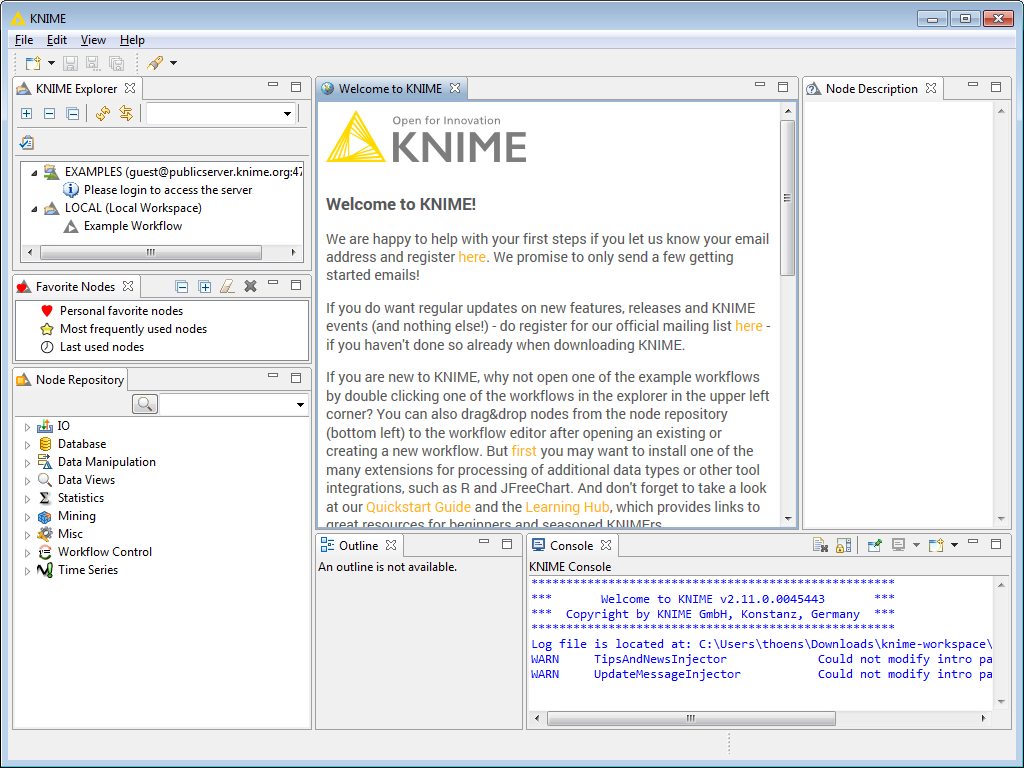
\includegraphics[height=0.6\textheight]{1.png}
	\end{center}
	\begin{itemize}
		\item The "KNIME Analytics Platform" must be installed before you can install FoodChain-Lab. Installation Instructions can be found at \url{https://tech.knime.org/installation-0}.
		\item When starting KNIME for the first time the interface looks like this.
	\end{itemize}
\end{frame}

\section{2}
\begin{frame}
	\begin{center}
  		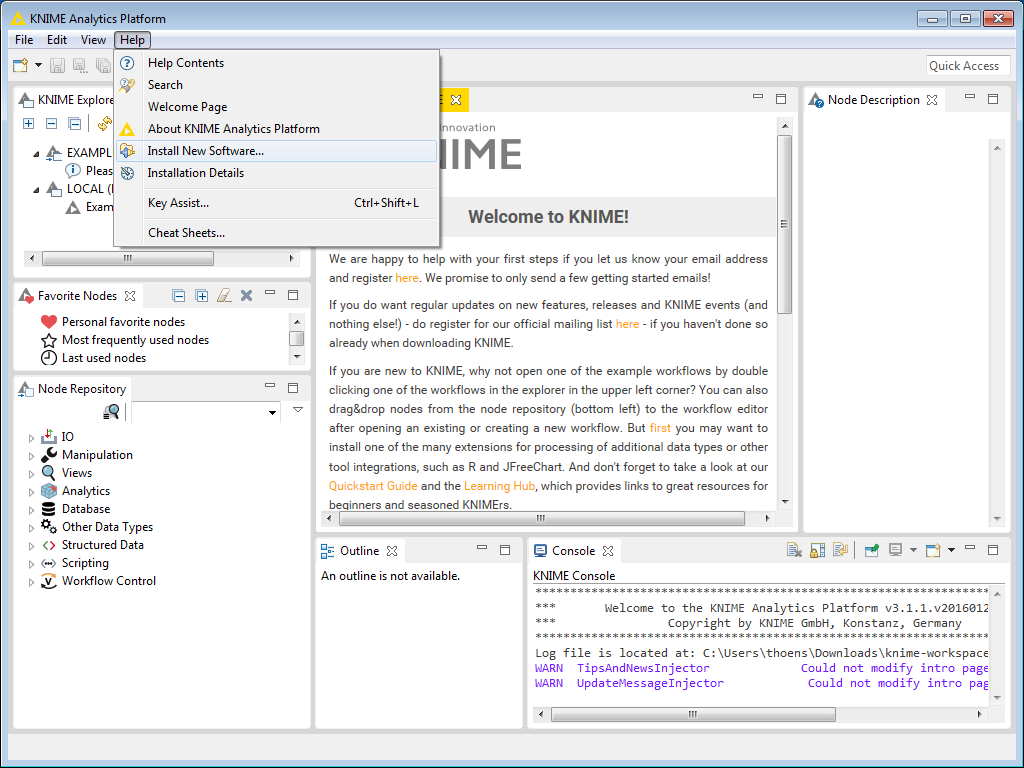
\includegraphics[height=0.7\textheight]{2.png}
	\end{center}
	\begin{itemize}
		\item Select \textbf{Help $>$ Install New Software} in the menu bar.
	\end{itemize}
\end{frame}

\section{3}
\begin{frame}
	\begin{center}
  		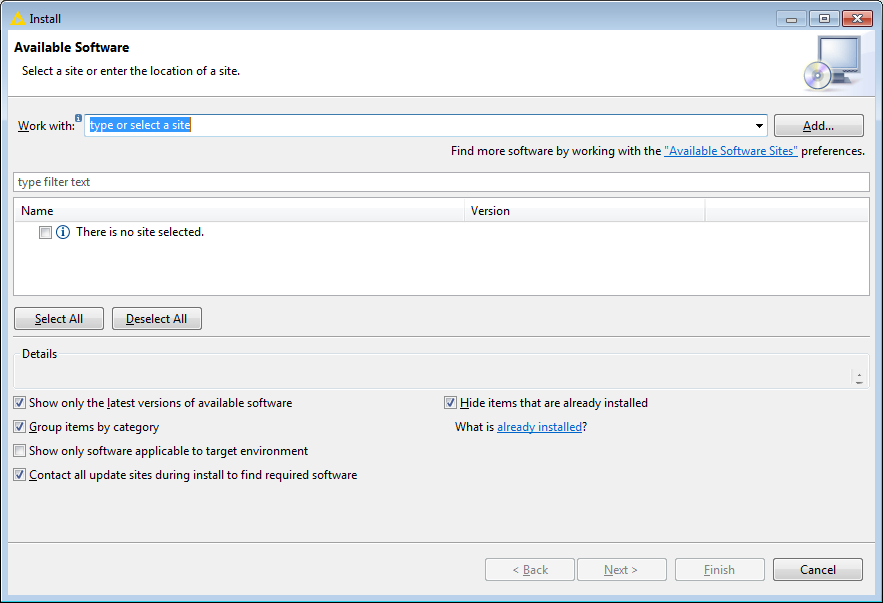
\includegraphics[height=0.7\textheight]{3.png}
	\end{center}
	\begin{itemize}
		\item Click \textbf{Add}, in the top-right corner.
	\end{itemize}
\end{frame}

\section{4}
\begin{frame}
	\begin{center}
  		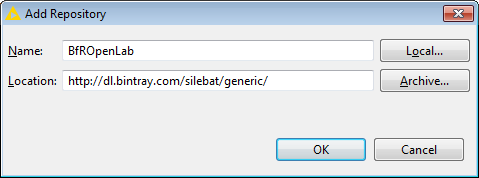
\includegraphics[width=0.9\textwidth]{4.png}
	\end{center}
	\begin{itemize}
		\item In the Add Repository dialog that appears, enter "BfROpenLab" for the \textit{Name} and the following URL for the \textit{Location}: \url{http://dl.bintray.com/silebat/generic/}
		\item Click \textbf{OK}.
	\end{itemize}
\end{frame}

\section{5}
\begin{frame}
	\begin{center}
  		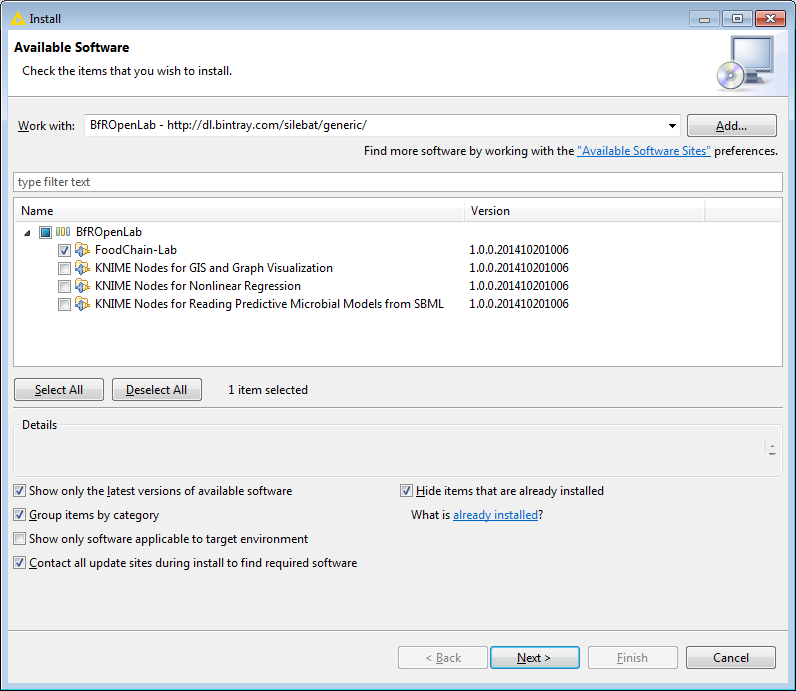
\includegraphics[height=0.7\textheight]{5.png}
	\end{center}
	\begin{itemize}
		\item In the Available Software dialog, expand the "BfROpenLab" entry and select the checkbox next to FoodChain-Lab.
		\item Click \textbf{Next}.
	\end{itemize}
\end{frame}

\section{6}
\begin{frame}
	\begin{center}
  		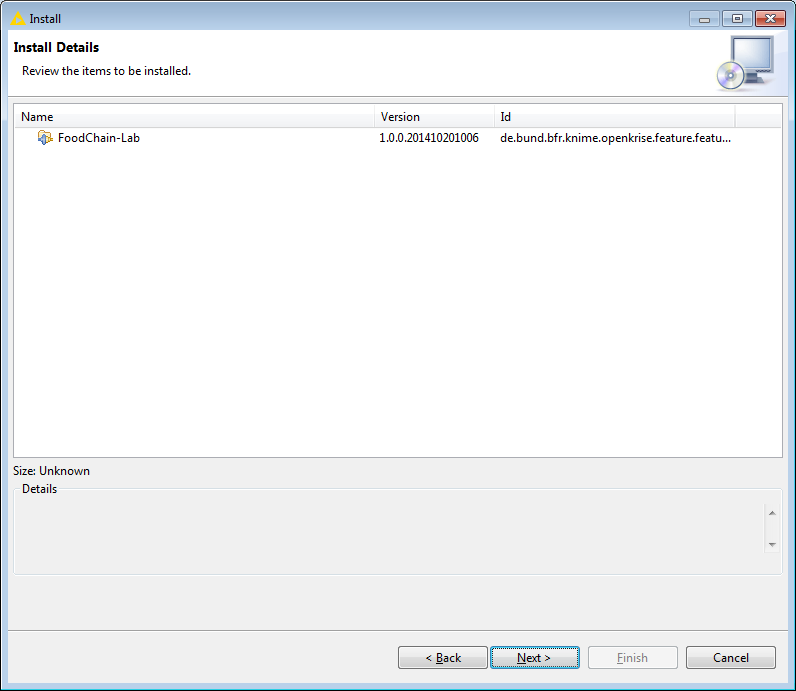
\includegraphics[height=0.7\textheight]{6.png}
	\end{center}
	\begin{itemize}
		\item In the next window, you'll see a list of the tools to be downloaded. Click \textbf{Next}.
	\end{itemize}
\end{frame}

\section{7}
\begin{frame}
	\begin{center}
  		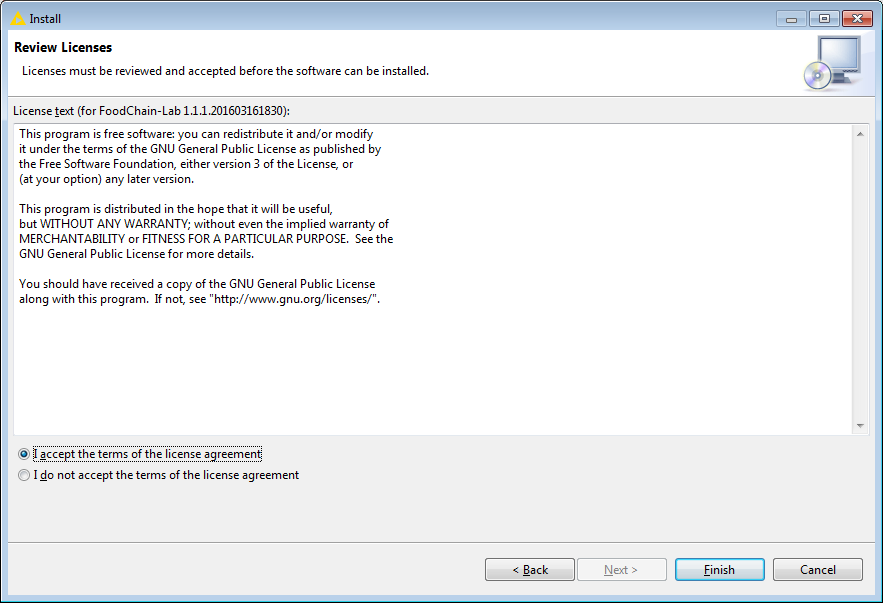
\includegraphics[width=0.7\textwidth]{7.png}
	\end{center}
	\begin{itemize}
		\item Read and accept the license agreements, then click \textbf{Finish}.
	\end{itemize}
\end{frame}

\section{8}
\begin{frame}
	\begin{center}
  		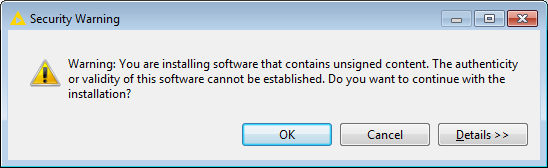
\includegraphics[width=0.9\textwidth]{8.png}
	\end{center}
	\begin{itemize}
		\item If you get a security warning saying that the authenticity or validity of the software can't be established, click \textbf{OK}.
	\end{itemize}
\end{frame}

\section{9}
\begin{frame}
	\begin{center}
  		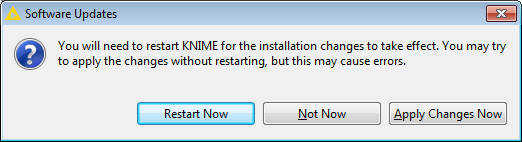
\includegraphics[width=0.9\textwidth]{9.png}
	\end{center}
	\begin{itemize}
		\item When the installation completes, restart KNIME.
	\end{itemize}
\end{frame}

\section{10}
\begin{frame}
	\begin{center}
  		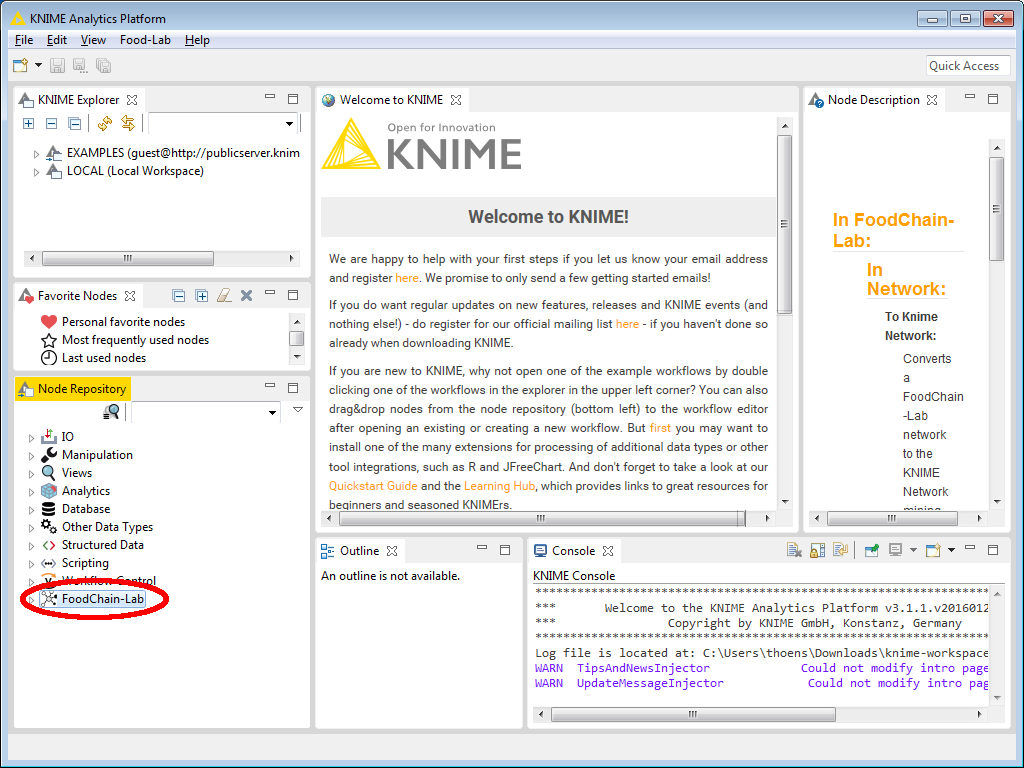
\includegraphics[height=0.6\textheight]{10.png}
	\end{center}
	\begin{itemize}
		\item When the KNIME interface has shown up, you should be able to see an item "FoodChain-Lab" in the \textbf{Node Repository} view in the bottom-left corner.
	\end{itemize}
\end{frame}

\end{document}